\documentclass[xcolor=pdftex,dvipsnames,table]{beamer}

\mode<presentation>
{
  \usetheme{Singapore}
  \usecolortheme{seahorse}
  \setbeamercovered{dynamic} %invisible
}

\usepackage[utf8]{inputenc}
\usepackage[english]{babel}
\usepackage{minted}

\usepackage{transparent}

\usepackage{tikz}
\usepackage{tikz-cd}
\usetikzlibrary{positioning}
% \def\checkmark{\tikz\fill[scale=0.4](0,.35) -- (.25,0) -- (1,.7) -- (.25,.15) -- cycle;}

\graphicspath{ {./images/} }

\def\checkmark{
\includegraphics[height=0.5cm]{checkmark}}
\def\crossmark{
\includegraphics[height=0.5cm]{crossmark}}
\def\questionmark{
\includegraphics[height=0.5cm]{question_mark}}

\definecolor{bgConsole}{HTML}{ffffcc}

\usepackage{tcolorbox}

\usepackage[absolute, overlay, showboxes]{textpos}
\TPGrid{16}{16}
\textblockorigin{0mm}{0mm}
\textblockrulecolour{bg}

%%%%%%%%%%%%%%%%%%%%%%%%%%%%%%

\title{Effect Handlers in Scope}
% \subtitle{}
\author[Wu, Schrijvers, Hinze]
{N.~Wu\inst{1} \and T.~Schrijvers\inst{2} \and R.~Hinze\inst{1}}

\institute[VFU] % (optional)
{
  \inst{1}%
  University of Oxford
  \and
  \inst{2}%
  Ghent University
}

\date[ICFP 2014]{ICFP 2014}

% \logo{
\includegraphics[height=0.5cm]{haskell-logo.png}}

%%%%%%%%%%%%%%%%%%%%%%%%%%%%%%

\AtBeginSection[]
{
  \begin{frame}<beamer>
      \frametitle{Table of Contents}
      \tableofcontents[currentsection]
  \end{frame}
}

\begin{document}

\frame{\titlepage}

\begin{frame}
  \begin{columns}[c]
    \column{0.4\textwidth}
    \begin{center}
      \Large{\textcolor{RoyalBlue}{Monad Transformers}}\\
      \small{Traditional Approach \\
      (Liang et al. 1995)}
    \end{center}

    \column{0.4\textwidth}
    \begin{center}
      \Large{\textcolor{ForestGreen}{Algebraic Effect Handlers}}\\
      \small{Recent Developments} \\
      \small{(Plotkin\&Power 2002, \\
      Kiselyov et al. 2013, \\
      Kammar et al. 2013, \\
      Brady 2013)}
    \end{center}
  \end{columns}
\end{frame}

\begin{frame}
  \begin{columns}[c]
    \column{0.3\textwidth}
    \begin{center}
      \Large{\textcolor{RoyalBlue}{Monad Transformers}}
    \end{center}
    \column{0.3\textwidth}
    \column{0.3\textwidth}
    \begin{center}
      \Large{\textcolor{ForestGreen}{Algebraic Effect Handlers}}
    \end{center}
  \end{columns}
  \bigskip
  \begin{columns}[c]
    \column{0.3\textwidth}
    \begin{center}
      \crossmark
    \end{center}
    \column{0.3\textwidth}
    \begin{center}
      \textbf{Methodology}
    \end{center}
    \column{0.3\textwidth}
    \begin{center}
      \checkmark
    \end{center}
  \end{columns}
  \begin{columns}[c]
    \column{0.3\textwidth}
    \begin{center}
      \crossmark
    \end{center}
    \column{0.3\textwidth}
    \begin{center}
      \textbf{Composition}
    \end{center}
    \column{0.3\textwidth}
    \begin{center}
      \checkmark
    \end{center}
  \end{columns}
\end{frame}

\begin{frame}
  \begin{columns}[c]
    \column{0.3\textwidth}
    \begin{center}
      \Large{\textcolor{RoyalBlue}{Monad Transformers}}
    \end{center}
    \column{0.3\textwidth}
    \column{0.3\textwidth}
    \begin{center}
      \Large{\textcolor{ForestGreen}{Algebraic Effect Handlers}}
    \end{center}
  \end{columns}
  \bigskip
  \bigskip
  \begin{columns}[c]
    \column{0.3\textwidth}
    \begin{center}
      \questionmark
    \end{center}
    \column{0.3\textwidth}
    \begin{center}
      \textbf{Effect Interaction}
    \end{center}
    \column{0.3\textwidth}
    \begin{center}
      \questionmark
    \end{center}
  \end{columns}
\end{frame}

{
\setbeamercolor{frametitle}{fg=white, bg=RoyalBlue}
\begin{frame}[fragile, t]
  \frametitle{Monad Transformers}
  \begin{center}
    \textbf{\Large{Effect Interaction?}}
  \end{center}
  \begin{minted}[bgcolor=bg, fontsize=\footnotesize]{haskell}
decr :: (MonadState Int m, MonadExcept () m)
     => m ()
decr = do x <- get
          if x > 0 then put (pred x)
                   else throw ()
  \end{minted}
  \pause
  \begin{minted}[bgcolor=bgConsole, fontsize=\footnotesize]{haskell}
ghci> (runId . runStateT 0 . runExceptT) decr
(Left (), 0)
  \end{minted}
  \pause
  \begin{minted}[bgcolor=bgConsole, fontsize=\footnotesize]{haskell}
ghci> (runId . runExceptT . runStateT 0) decr
Left ()
  \end{minted}

  {
  \TPMargin{2mm}
  \textblockcolour{RoyalBlue}
    \only<4>{
      \begin{textblock}{8}(4,5)
        \vspace{5mm}
        \begin{minipage}{0.2\textwidth}
          
\includegraphics[height=1cm]{okhand}
        \end{minipage}
        \begin{minipage}{0.7\textwidth}
          \begin{center}
          Effect interaction \`a la carte!
          \end{center}
        \end{minipage}
        \vspace{5mm}
      \end{textblock}
    }
  }
\end{frame}
}

\begin{frame}
  \begin{columns}[c]
    \column{0.3\textwidth}
    \begin{center}
      \Large{\textcolor{RoyalBlue}{Monad Transformers}}
    \end{center}
    \column{0.3\textwidth}
    \column{0.3\textwidth}
    \begin{center}
      \Large{\textcolor{ForestGreen}{Algebraic Effect Handlers}}
    \end{center}
  \end{columns}
  \bigskip
  \bigskip
  \begin{columns}[c]
    \column{0.3\textwidth}
    \begin{center}
      \checkmark
    \end{center}
    \column{0.3\textwidth}
    \begin{center}
      \textbf{Effect Interaction}
    \end{center}
    \column{0.3\textwidth}
    \begin{center}
      \questionmark
    \end{center}
  \end{columns}
\end{frame}

{
\setbeamercolor{frametitle}{fg=white, bg=ForestGreen}
\begin{frame}[fragile, t]
  \frametitle{Algebraic Effect Handlers}
  \begin{center}
    \textbf{\Large{Effect Interaction?}}
  \end{center}
  \begin{minted}[bgcolor=bg, fontsize=\footnotesize]{haskell}
decr :: (State Int <: sig, Exc () <: sig)
     => Prog sig ()
decr = do x <- get
          if x > 0 then put (pred x)
                    else throw ()
  \end{minted}
  \pause
  \begin{minted}[bgcolor=bgConsole,fontsize=\footnotesize]{haskell}
ghci> (run . runState 0 . runErr) decr
(Left (), 0)
  \end{minted}
  \pause
  \begin{minted}[bgcolor=bgConsole, fontsize=\footnotesize]{haskell}
ghci> (run . runErr . runState 0) decr
Left ()
  \end{minted}

  {
  \TPMargin{2mm}
  \textblockcolour{ForestGreen}
    \only<4>{
      \begin{textblock}{8}(4,5)
        \vspace{5mm}
        \begin{minipage}{0.2\textwidth}
          
\includegraphics[height=1cm]{okhand}
        \end{minipage}
        \begin{minipage}{0.7\textwidth}
          \begin{center}
          Effect interaction \`a la carte!
          \end{center}
        \end{minipage}
        \vspace{5mm}
      \end{textblock}
    }
  }
\end{frame}
}

\begin{frame}
  \begin{columns}[c]
    \column{0.3\textwidth}
    \begin{center}
      \Large{\textcolor{RoyalBlue}{Monad Transformers}}
    \end{center}
    \column{0.3\textwidth}
    \column{0.3\textwidth}
    \begin{center}
      \Large{\textcolor{ForestGreen}{Algebraic Effect Handlers}}
    \end{center}
  \end{columns}
  \bigskip
  \bigskip
  \begin{columns}[c]
    \column{0.3\textwidth}
    \begin{center}
      \checkmark
    \end{center}
    \column{0.3\textwidth}
    \begin{center}
      \textbf{Effect Interaction}
    \end{center}
    \column{0.3\textwidth}
    \begin{center}
      \checkmark
    \end{center}
  \end{columns}
\end{frame}

\begin{frame}[fragile]
  \begin{center}
    \textbf{\Large{Effect Interaction with \\ Scoping Constructs}}
  \end{center}
  \bigskip
  \begin{minted}[bgcolor=bg, fontsize=\large, escapeinside=||]{haskell}
tripleDecr = decr >> |\color{red}{catch}| (decr >> decr) return
  \end{minted}
\end{frame}

\begin{frame}[fragile]
  \begin{center}
    \textbf{\Large{Effect Interaction with \\ Scoping Constructs}}
    \bigskip
    \begin{minted}[bgcolor=bg, fontsize=\footnotesize, escapeinside=||]{haskell}
      tripleDecr = decr >> |\color{red}{catch}| (decr >> decr) return
    \end{minted}
    {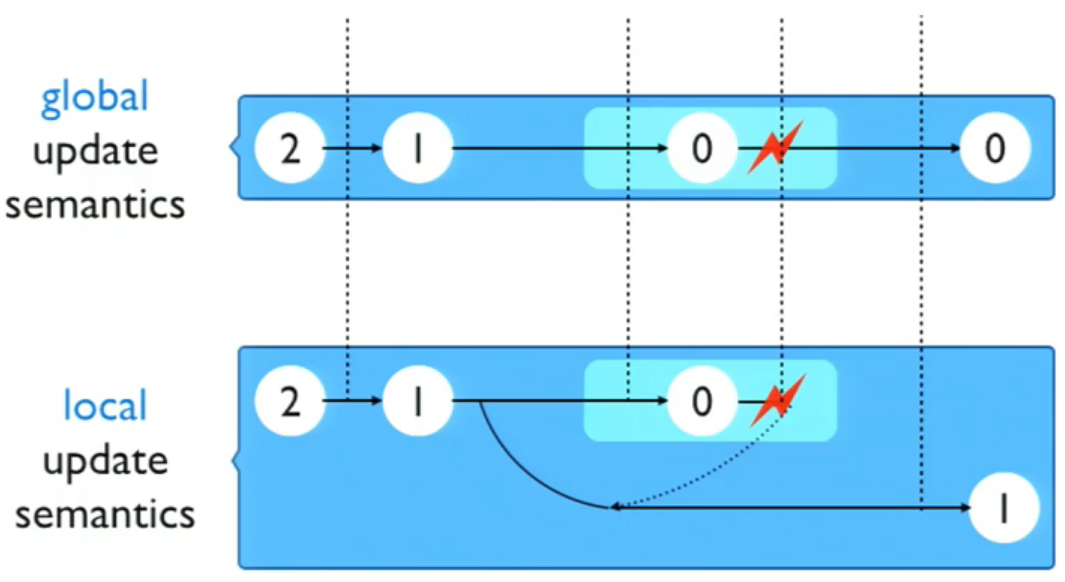
\includegraphics[scale=0.30]{interactions.png}}
  \end{center}
\end{frame}

{
\setbeamercolor{frametitle}{fg=white, bg=RoyalBlue}
\setbeamercovered{invisible}
\TPMargin{1pt}
\setlength{\TPboxrulesize}{1pt}

\begin{frame}[fragile, t]
  \frametitle{Monad Transformers}
  \begin{center}
    \textbf{\Large{Global Updates?}} \\
    \textbf{\Large{Local Updates?}}
  \end{center}

  \onslide<1->
  \begin{minted}[bgcolor=bg, fontsize=\footnotesize, escapeinside=||]{haskell}
tripleDecr :: (MonadState Int m, MonadExcept () m)
           => m ()
tripleDecr = decr >> |\color{red}{catch}| (decr >> decr) return
  \end{minted}

  \onslide<2->
  \begin{minted}[bgcolor=bgConsole, fontsize=\footnotesize]{haskell}
ghci> (runId . runStateT 2 . runExceptT) tripleDecr
(Right (), 0)
  \end{minted}

  \only<3->{
    \textblockcolour{Cyan}
    \textblockrulecolour{RoyalBlue}
    \begin{textblock}{4}(5,10.5)
      \begin{center}
        \footnotesize\textbf{\color{White}{global update}}
      \end{center}
    \end{textblock}
  }

  \only<4->{
    \textblockcolour{bg}
    \textblockrulecolour{bg}
    \begin{textblock}{2}(10.5,3.2)
      \checkmark
    \end{textblock}
  }

  \bigskip

  \onslide<5->
  \begin{minted}[bgcolor=bgConsole, fontsize=\footnotesize]{haskell}
ghci> (runId . runExceptT . runStateT 2) tripleDecr
Right ((), 1)
  \end{minted}

  \only<6->{
    \textblockcolour{Cyan}
    \textblockrulecolour{RoyalBlue}
    \begin{textblock}{4}(5,13.5)
      \begin{center}
        \footnotesize\textbf{\color{White}{local update}}
      \end{center}
    \end{textblock}
  }

  \only<7->{
    \textblockcolour{bg}
    \textblockrulecolour{bg}
    \begin{textblock}{2}(10.5,4.2)
      \checkmark
    \end{textblock}
  }

\end{frame}
}

\begin{frame}
  \begin{columns}[c]
    \column{0.3\textwidth}
    \begin{center}
      \Large{\textcolor{RoyalBlue}{Monad Transformers}}
    \end{center}
    \column{0.3\textwidth}
    \column{0.3\textwidth}
    \begin{center}
      \Large{\textcolor{ForestGreen}{Algebraic Effect Handlers}}
    \end{center}
  \end{columns}
  \bigskip
  \bigskip
  \begin{columns}[c]
    \column{0.3\textwidth}
    \begin{center}
      \checkmark
      \checkmark
    \end{center}
    \column{0.3\textwidth}
    \begin{center}
      \textbf{Effect Interaction}
    \end{center}
    \column{0.3\textwidth}
    \begin{center}
      \checkmark
      \questionmark
    \end{center}
  \end{columns}
\end{frame}

{
\setbeamercolor{frametitle}{fg=white, bg=ForestGreen}
\setbeamercovered{invisible}
\TPMargin{1pt}
\setlength{\TPboxrulesize}{1pt}

\begin{frame}[fragile, t]
  \frametitle{Algebraic Effect Handlers}
  \begin{center}
    \textbf{\Large{Global Updates?}} \\
    \textbf{\Large{Local Updates?}}
  \end{center}

  \onslide<1->
  \begin{minted}[bgcolor=bg, fontsize=\footnotesize, escapeinside=||]{haskell}
tripleDecr :: (State Int <: sig, Exc () <: sig)
           => Prog sig ()
tripleDecr = decr >> |\color{red}{catch}| (decr >> decr) return
  \end{minted}

  \onslide<1->
  \begin{minted}[bgcolor=bgConsole, fontsize=\footnotesize]{haskell}
ghci> (run . runState 2 . runExc) tripleDecr
(Right (), 0)
  \end{minted}

  \only<2->{
    \textblockcolour{Green}
    \textblockrulecolour{ForestGreen}
    \begin{textblock}{4}(5,10.5)
      \begin{center}
        \footnotesize\textbf{\color{White}{global update}}
      \end{center}
    \end{textblock}
  }

  \only<2->{
    \textblockcolour{bg}
    \textblockrulecolour{bg}
    \begin{textblock}{2}(10.5,3.2)
      \checkmark
    \end{textblock}
  }

  \bigskip

  \onslide<3->
  \begin{minted}[bgcolor=bgConsole, fontsize=\footnotesize]{haskell}
ghci> (run . runExc . runState 2) tripleDecr
Right ((), 0)
  \end{minted}

  \only<4->{
    \textblockcolour{Red}
    \textblockrulecolour{BrickRed}
    \begin{textblock}{4}(5,13.5)
      \begin{center}
        \footnotesize\textbf{\color{White}{global update}}
      \end{center}
    \end{textblock}
  }

  \only<4->{
    \textblockcolour{bg}
    \textblockrulecolour{bg}
    \begin{textblock}{2}(10.5,4.2)
      \crossmark
    \end{textblock}
  }

\end{frame}
}

\begin{frame}
  \begin{center}
   \textbf{\color{RoyalBlue}{\LARGE{Why is Catch Different?}}}
  \end{center}
\end{frame}

\begin{frame}[fragile,t]
  \begin{center}
    \textbf{\Large{Effect Handlers}}
  \end{center}
  \bigskip
  % \begin{tikzpicture}[node distance = 2cm, thick]%
  %     \node (1) {atomic operations \\ (get/put/throw/\ldots)};
  %     \node (5) [below=of 1] {};
  %     \node (4) [below=of 5] {};
  %     \node (2) [left=of 4] {\color{RoyalBlue}{syntax\\(functor)}};
  %     \node (3) [right=of 4] {\color{ForestGreen}{semantics\\=\\handler function}};
  %     \draw[->] (5) -- node [midway,above] {} (2);
  %     \draw[->] (5) -- node [midway,above] {} (3);
  %     \draw [dashed] (1) -- (4);
  % \end{tikzpicture}%

  \only<1>{
  \begin{center}
    atomic operations \\
    (get/put/throw/\ldots)
  \end{center}
  \begin{columns}[c]
    \column{0.2\textwidth}
    \column{0.2\textwidth}
    \begin{center}
      \color{RoyalBlue}{syntax\\(functor)}
    \end{center}

    \column{0.2\textwidth}
    \begin{center}
      \begin{tikzpicture}[node distance = 3cm, thick]%
          \node (1) {};
          \node (2) [below=of 1] {};
          \draw [dashed] (1) -- (2);
      \end{tikzpicture}%
    \end{center}

    \column{0.2\textwidth}
    \begin{center}
      \color{ForestGreen}{semantics\\=\\handler function}
    \end{center}
    \column{0.2\textwidth}
  \end{columns}
  }

  \only<2-3>{
  \begin{center}
    \textcolor{red}{scoping} operations \\
    (e.g., catch)
  \end{center}
  \begin{columns}[c]
    \column{0.2\textwidth}
    \column{0.2\textwidth}
    \begin{center}
      \color{RoyalBlue}{scope\\=\\syntax}
    \end{center}

    \column{0.2\textwidth}
    \begin{center}
      \begin{tikzpicture}[node distance = 3cm, thick]%
          \node (1) {};
          \node (2) [below=of 1] {};
          \draw [dashed] (1) -- (2);
      \end{tikzpicture}%
    \end{center}

    \column{0.2\textwidth}
    \begin{center}
      \color{ForestGreen}{semantics\\=\\handler function}
    \end{center}
    \column{0.2\textwidth}
  \end{columns}
  }


  \only<3>{
    \textblockcolour{bg}
    \textblockrulecolour{bg}
    \begin{textblock}{2}(2,10.5)
      
\includegraphics[height=1cm]{crossmark}
    \end{textblock}
    \textblockcolour{bg}
    \textblockrulecolour{bg}
    \begin{textblock}{4}(1,12.5)
      \textcolor{red}{shape does not fit}
    \end{textblock}
  }

  \only<4->{
  \begin{center}
    \textcolor{red}{scoping} operations \\
    (e.g., catch)
  \end{center}
  \begin{columns}[c]
    \column{0.2\textwidth}
    \column{0.2\textwidth}

    \column{0.2\textwidth}
    \begin{center}
      \begin{tikzpicture}[node distance = 3cm, thick]%
          \node (1) {};
          \node (2) [below=of 1] {};
          \draw [dashed] (1) -- (2);
      \end{tikzpicture}%
    \end{center}

    \column{0.2\textwidth}
    \begin{center}
      \color{ForestGreen}{semantics\&scope\\=\\handler function}
    \end{center}
    \column{0.2\textwidth}
  \end{columns}
  }
\end{frame}


\begin{frame}[fragile,t]
  \begin{center}
    \textbf{\Large{This paper}}
  \end{center}
  \bigskip

  \only<1>{
  \begin{center}
    \textcolor{red}{scoping} construct \\
    (e.g., catch)
  \end{center}
  \begin{columns}[c]
    \column{0.2\textwidth}
    \column{0.2\textwidth}
    \begin{center}
      \color{RoyalBlue}{scope\\=\\syntax}
    \end{center}

    \column{0.2\textwidth}
    \begin{center}
      \begin{tikzpicture}[node distance = 3cm, thick]%
          \node (1) {};
          \node (2) [below=of 1] {};
          \draw [dashed] (1) -- (2);
      \end{tikzpicture}%
    \end{center}

    \column{0.2\textwidth}
    \begin{center}
      \color{ForestGreen}{semantics\\=\\handler}
    \end{center}
    \column{0.2\textwidth}
  \end{columns}
  }
\end{frame}

\begin{frame}
  \begin{center}
   \textbf{\color{RoyalBlue}{\LARGE{Solution: \\ Higher-Order Syntax}}}
  \end{center}
\end{frame}

\begin{frame}[t, fragile]
  \begin{center}
    \textbf{\Large{First-Order Syntax}}
  \end{center}
  \begin{minted}[bgcolor=bg, fontsize=\footnotesize]{haskell}
data Exc e cnt
    = Throw' e
  deriving (Functor)

data Catch e cnt
    = BCatch' cnt (e -> cnt)
    | ECatch' cnt
  deriving (Functor)
  \end{minted}
  \begin{center}
    \textbf{\Large{Higher-Order Syntax}}
  \end{center}
  \begin{minted}[bgcolor=bg, fontsize=\footnotesize]{haskell}
data HExc e m a
  = Throw' e
  | forall x. Catch' (m x) (e -> m x) (x -> m a)
  \end{minted}
\end{frame}

\begin{frame}[t, fragile]
  \begin{center}
    \textbf{\Large{Implications of \\ Higher-Order Syntax}}
  \end{center}
  \bigskip
  \begin{itemize}
      \item \textcolor{RoyalBlue}{Syntax:}\\ higher-order functors
      \item \textcolor{RoyalBlue}{Free monad infrastructure:}\\ for higher-order functors
      \item \textcolor{RoyalBlue}{Handlers:}\\ compositional semantics satisfying a distributive property
  \end{itemize}

  \only<2>{
    \setlength{\TPboxrulesize}{2pt}
    \textblockcolour{ForestGreen}
    \textblockrulecolour{ForestGreen}
    \begin{textblock}{3}(9,6)
      \begin{center}
        \textbf{\color{White}{See \\ the paper}}
      \end{center}
    \end{textblock}
  }
\end{frame}

\begin{frame}[fragile, t]
  \begin{center}
    \textbf{\Large{Global Updates?}} \\
    \textbf{\Large{Local Updates?}}
  \end{center}

  \begin{minted}[bgcolor=bg, fontsize=\footnotesize, escapeinside=||]{haskell}
tripleDecr :: (State Int <: sig, Exc () <: sig)
           => Prog sig ()
tripleDecr = decr >> |\color{red}{catch}| (decr >> decr) return
  \end{minted}

  \onslide<1->
  \begin{minted}[bgcolor=bgConsole, fontsize=\footnotesize]{haskell}
ghci> (run . runState 2 . runExc) tripleDecr
(Right (), 0)
  \end{minted}

  {
    \textblockcolour{Green}
    \textblockrulecolour{ForestGreen}
    \begin{textblock}{4}(5,8.6)
      \begin{center}
        \footnotesize\textbf{\color{White}{global update}}
      \end{center}
    \end{textblock}
  }

  {
    \textblockcolour{bg}
    \textblockrulecolour{bg}
    \begin{textblock}{2}(10.5,1.5)
      \checkmark
    \end{textblock}
  }

  \bigskip

  \begin{minted}[bgcolor=bgConsole, fontsize=\footnotesize]{haskell}
ghci> (run . runExc . runState 2) tripleDecr
Right ((), 1)
  \end{minted}

  {
    \textblockcolour{Green}
    \textblockrulecolour{ForestGreen}
    \begin{textblock}{4}(5,11.5)
      \begin{center}
        \footnotesize\textbf{\color{White}{local update}}
      \end{center}
    \end{textblock}
  }

  {
    \textblockcolour{bg}
    \textblockrulecolour{bg}
    \begin{textblock}{2}(10.5,2.8)
      \checkmark
    \end{textblock}
  }

\end{frame}

%%%%%%%%%%%%%%%%%%%

\begin{thebibliography}{5}
  % \bibitem{Goldbach1742}[Goldbach, 1742]
  % Christian Goldbach.
  % \newblock A problem we should try to solve
\end{thebibliography}

%%%%%%%%%%%%%%%%%%%%%

\end{document}

